\documentclass[11pt]{article}

% \usepackage{}
\usepackage{amssymb,amsmath,amsfonts,eurosym,geometry,ulem,graphicx,caption,color,setspace,sectsty,comment,footmisc,caption,natbib,pdflscape,array,hyperref,caption,subcaption}

\normalem

\onehalfspacing
\newtheorem{theorem}{Theorem}
\newtheorem{corollary}[theorem]{Corollary}
\newtheorem{proposition}{Proposition}
\newenvironment{proof}[1][Proof]{\noindent\textbf{#1.} }{\ \rule{0.5em}{0.5em}}

\newtheorem{hyp}{Hypothesis}
\newtheorem{subhyp}{Hypothesis}[hyp]
\renewcommand{\thesubhyp}{\thehyp\alph{subhyp}}

\newcommand{\red}[1]{{\color{red} #1}}
\newcommand{\blue}[1]{{\color{blue} #1}}

\newcolumntype{L}[1]{>{\raggedright\let\newline\\arraybackslash\hspace{0pt}}m{#1}}
\newcolumntype{C}[1]{>{\centering\let\newline\\arraybackslash\hspace{0pt}}m{#1}}
\newcolumntype{R}[1]{>{\raggedleft\let\newline\\arraybackslash\hspace{0pt}}m{#1}}

\geometry{left=1.0in,right=1.0in,top=1.0in,bottom=1.0in}


\begin{document}
\begin{titlepage}
\title{\textbf{Property Division, Housing Registration, and Intra-household Bargaining Power: Evidence from China}}
\author{Yuhao Zhang}
\date{May 2023}
\maketitle
\begin{abstract}
\noindent Placeholder\\
\vspace{0in}\\
\noindent\textbf{Keywords:} key1, key2, key3\\
\vspace{0in}\\
\noindent\textbf{JEL Codes:} key1, key2, key3\\

\bigskip
\end{abstract}
\setcounter{page}{0}
\thispagestyle{empty}
\end{titlepage}
\pagebreak \newpage


\section{Introduction} \label{sec:intro}
A number of studies explore the impact of changes in housing, a major component of marriage-and-family-related matters in China, on marriage and household behavior. For one thing, traditional notions emphasize housing as the material root of a family. For another thing, the housing market in China has experienced a dramatic boom in the past decades, which has led to a significant increase in housing prices, rendering housing purchase a major challenge for the new couples to conquer.

In 2011, the Supreme Court of China announced a new statutory interpretation of \textit{the Marriage Law} in terms of several issues upon property division after a divorce. Among these, \textbf{one of the} most noticeable changes is that the housing purchased by either spouse before marriage, or the housing the down payment of which was paid by one spouse and registered solely with his/her name, is no longer considered as a joint property of the couple. Instead, it is considered as a personal property, or only the mortgage loan paid with the common wealth after marriage will be transformed into debt. The court can justifiably say that the housing should belong to its nominal owner. \textbf{In addition}, the housing bought by either spouse's parents and registered with this child's name after marriage should only be deemed as a gift instead of the couple's joint property.

These new instructions were bound to have great impacts on Chinese families. Some regard this interpretation as a severe violation of women's rights, since it encourages men to divorce their wives with litigation without losing their properties. \footnote{As we will see later, before 2011, half of the families in our sample registered their housing under the husbands' names} Therefore, it is highly possible that a man will have a stronger bargaining power in the family, since the outside option of the female is quite determined by him. On the other hand, however, wives can strive to put their names on the license to maximize their benefits, which again depends on \textbf{their} bargaining power. Their mutual determination of each other, for one thing, complicates our research on the impact of the reform, but, for another things, it illustrates the intricacies of bargaining power and economic behaviors within Chinese families.

Based on (Inspired by) this new judicial interpretation, our research examines how the housing registration of Chinese families evolve during the past decade and how it is related to the intra-household bargaining power and other features. Furthermore, we put this into the context of the incredibly booming property market in China, which should be a major consideration for both singles and married couples when making decisions.

Overall, in our sample, the proportion of couples who list both the husband and the wife on the license significantly increases, with husband-registered houses accounting for over 50\% of the houses initially but less and less henceforth. The proportion of houses registered under the wife's name does not have a robust trend of changing. There is also a flow from parents-registered houses to co-owned houses, which is consistent with the fact that the new judicial interpretation also considers the former as a gift to one side of the couple.

\section{Literature Review} \label{sec:literature}
\citet{SUN2020102492} mainly examined how the surging housing price reinforces assortative mating (raising the years of education of wives). As a robustness test, however, the new judicial interpretation was found to lower such sorting since there is fewer expected benefits to attract the well-educated females to marry with men. (This can also be attributed partly to the change in bargaining power arrangements after marriage).

\citet{WANG2014192} solely focused on this interpretation and examined its impact on intra-household behavior 
with a difference-in-differences approach. Naturally, they set the treatment group to be those who bought houses \textbf{before} marriage whereas the control group to be those who purchased \textbf{after} the marriage, among whom the former group has a higher probability to exclude the wife's name out of the license. They found that the males who bought houses before marriage tended more to smoke and drink excessively, while their wives had less leisure time and their children got fewer resources in human capital investments. 

In this study, we try to make some subtle contribution to these studies by examining how the rising housing price and marital property right reform jointly affect the pattern of housing registration. Although the analysis not necessarily in a causal sense, it provides important descriptive evidence for the change in housing registration and its correlation with other variables.


\section{Data} \label{sec:data}

China Family Panel Studies (CFPS), a major representative panel survey on Chinese families, which collected abundant information from residents in terms of their family configuration, economic status, personal history, etc. Fortunately, we are able to track many households' housing registration information from 2010 to 2018, which is the main data source for our research.

In addition, variables on other characteristics are surveyed in CFPS, such as individuals' ages, genders, income, etc. The macro housing price data are at provincial level and are obtained from the website of National Bureau of Statistics (\href{https://data.stats.gov.cn/easyquery.htm?cn=E0103}{https://data.stats.gov.cn/easyquery.htm?cn=E0103}).

\section{Empirical Design and Results} \label{sec:method}

\subsection{Descriptive Analysis}

We first provide some descriptive evidence on the change of housing registration, mainly using the \textit{Sankey plot}, which is a type of flow diagram that visualizes the flow of data between a set of nodes. In our case, the nodes are the different types of housing registration, and the flow is the number of households that shift from one type to another.

\begin{figure}
    \centering
    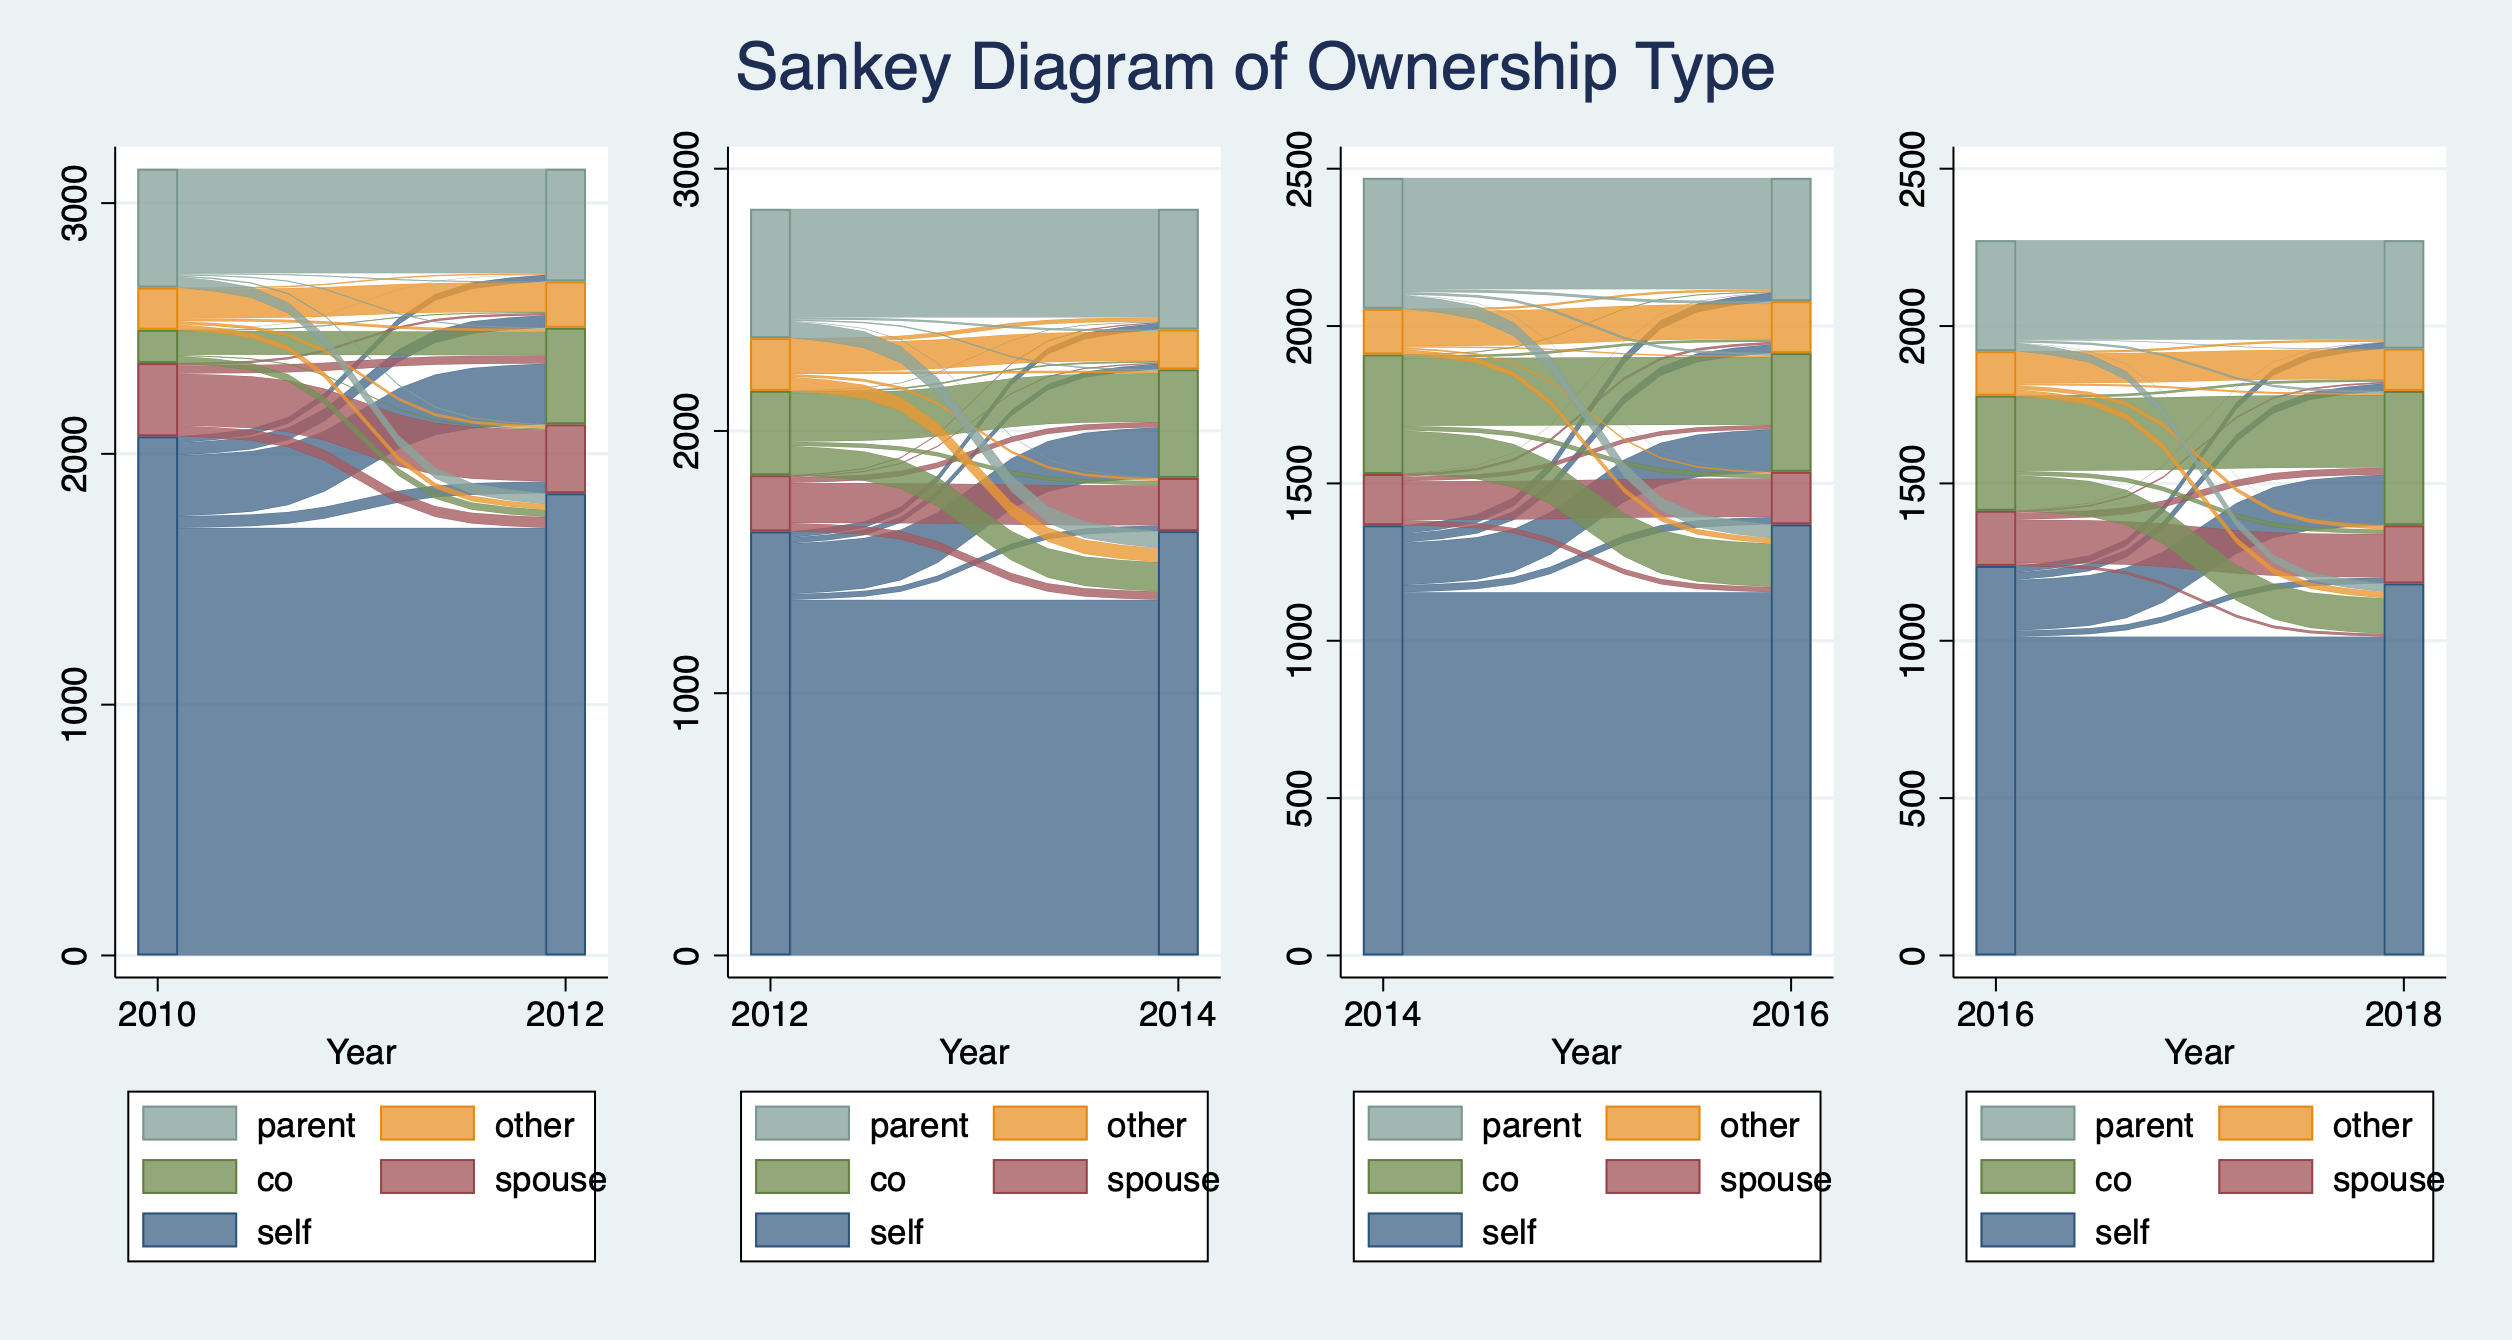
\includegraphics[width = \textwidth]{./graphs_new/sankeyall_nonpanel.png}
    \caption{Non Panel}
    \label{fig:sankeyall_nonpanel}
\end{figure}

In Figure \ref{fig:sankeyall_nonpanel}, I divide the sample into pairs of adjacent waves. This is because there are rarely families appearing in all the waves of surveys, and we can instead look at neighboring waves to see the change in housing registration. Note that in the legend, ``self'' refers to the husband and ``spouse'' refers to the wife.

From 2010 to 2012, the proportion of co-owned housing has saliently risen, a large part of which is contributed by the converted husband-owned housing. Despite some increase in co-owned proportion in the following years, there are also a lot of families change their joint registration to a husband-owned one. The proportion of wife-owned and parent-owned housing are relatively stable. These pieces of evidence indicate the possible impact of the interpretation on how families register their houses as well as how highly Chinese families value their housing. Another implication is that people do care about ``outside option'', even if Chinese traditional culture regards divorce as a taboo in discourse.

\begin{figure}
    \centering
    \begin{subfigure}[b]{0.45\textwidth}
        \centering
        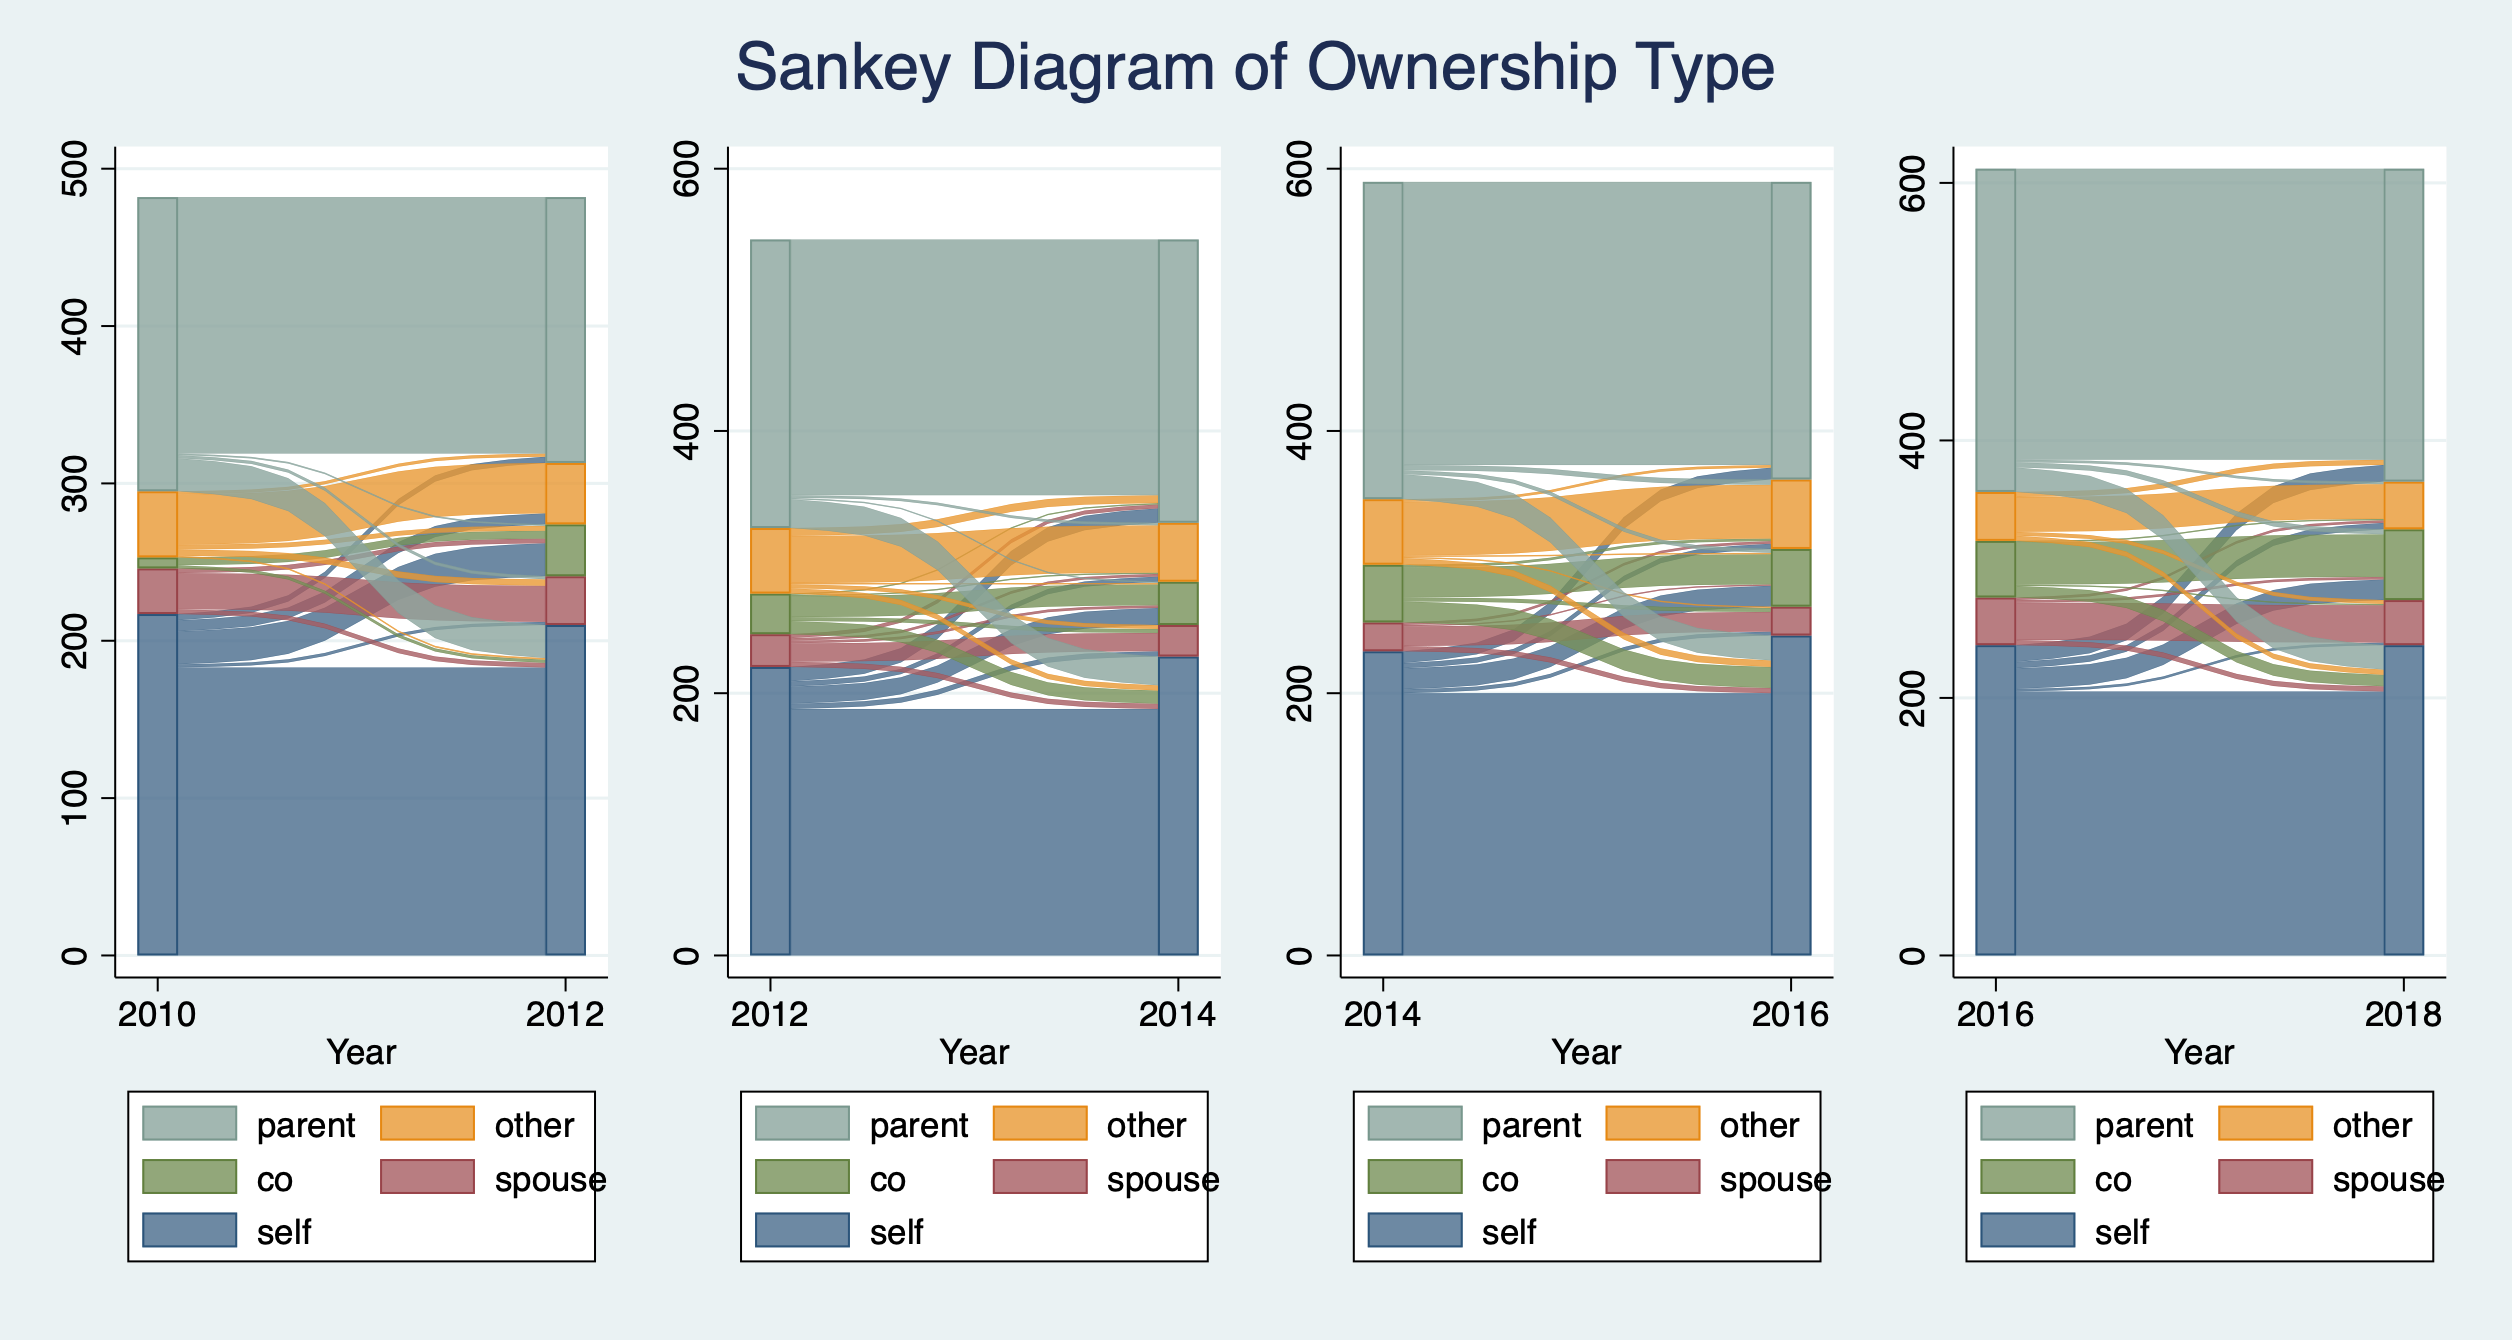
\includegraphics[width=\textwidth]{graphs_new/pbeforem_sankeyall_nonpanel.png}
        \caption{Purchase before marriage}
        \label{fig:pbeforem}
        
    \end{subfigure}
    \hfill
    \begin{subfigure}[b]{0.45\textwidth}
        \centering
        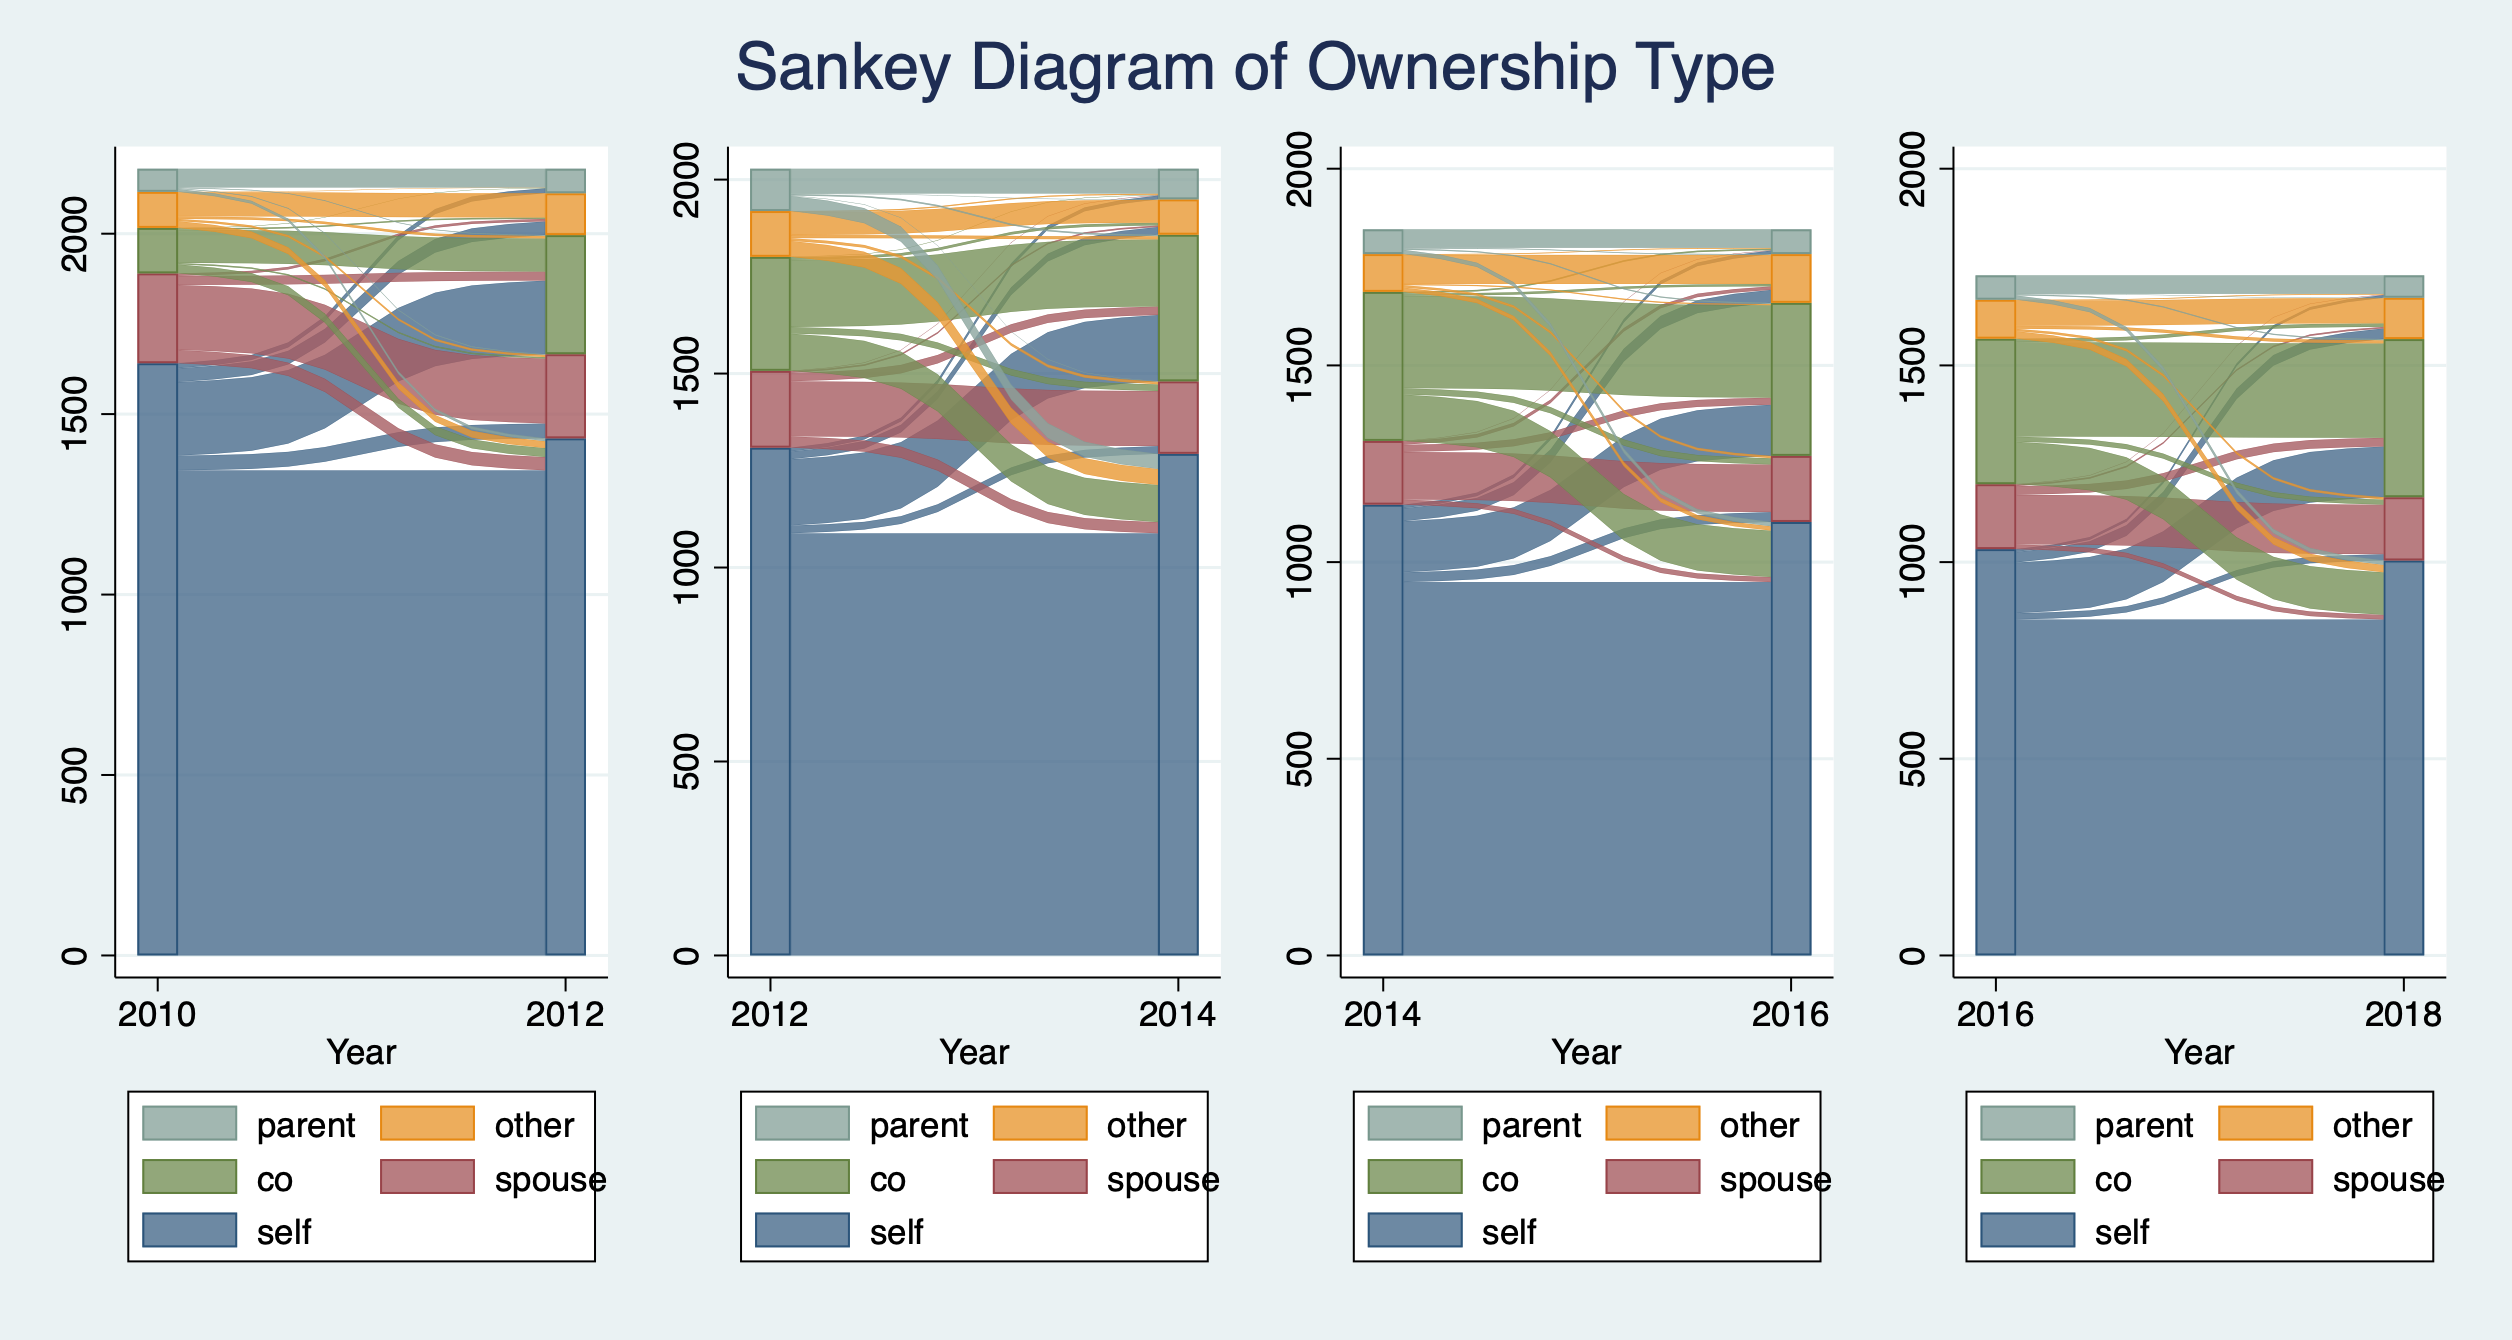
\includegraphics[width=\textwidth]{graphs_new/pafterm_sankeyall_nonpanel.png}
        \subcaption{Purchase after marriage}
        \label{fig:pafterm}
        
    \end{subfigure}
    \caption{Sankey Diagram according to the timing of purchase}
    \label{fig:timing}
\end{figure}

Figure \ref{fig:timing} tells us more about the possible impact of the interpretation. We divide the families into those who purchased their housing before marriage and the other. According to \citet{Huang532}, those who purchase housing before marriage, typically buying the house using one's or one's parents' money and registering it under only that person's name, are more likely to be affected by the interpretation. However, we even see a more drastic increase in co-owned housing among those who purchase after marriage. As for those who bought houses before marriage, their parents contribute much to the purchase and transfer the ownership to their children after 2010. Of course, the weight of co-ownership also increases among them.

\subsection{Mechanisms}

To explore the correlation between family characteristics and the shift in housing registration, we use multiple Logistic regression model to see the impact of each variable on the probability of the registration being each kind. We cannot capture the change from multiple states to multiple states, so this analysis is restricted to those who initially have a husband-owned house in one wave as well as the same group of people in the next wave. 

\begin{table}[h]
    \centering
    
\begin{tabular}{l*{5}{c}}
    \hline\hline
                &\multicolumn{1}{c}{(1)}&\multicolumn{1}{c}{(2)}&\multicolumn{1}{c}{(3)}&\multicolumn{1}{c}{(4)}&\multicolumn{1}{c}{(5)}\\
                &\multicolumn{1}{c}{edu\_w} &\multicolumn{1}{c}{edu} &\multicolumn{1}{c}{marriage year} &\multicolumn{1}{c}{purchase year} &\multicolumn{1}{c}{ln(income)} \\
    \hline
            &                     &                     &                     &                     &                     \\
    1. husband  &      -0.013{***}&       0.001         &      -0.008{***}&      -0.004{***}&      -0.003         \\
                &     (0.003)         &     (0.003)         &     (0.002)         &     (0.001)         &     (0.002)         \\
    [1em]
    2. wife  &       0.008{***}&       0.000         &       0.003{**} &       0.002{**} &       0.002         \\
                &     (0.002)         &     (0.002)         &     (0.001)         &     (0.001)         &     (0.001)         \\
    [1em]
    3. co-owned  &       0.006{**} &       0.002         &       0.000         &       0.004{***}&       0.002         \\
                &     (0.002)         &     (0.002)         &     (0.001)         &     (0.001)         &     (0.002)         \\
    [1em]
    4. others  &       0.001         &      -0.001         &       0.002{*}  &       0.001{*}  &      -0.001         \\
                &     (0.001)         &     (0.001)         &     (0.001)         &     (0.001)         &     (0.001)         \\
    [1em]
    5. parents  &      -0.002         &      -0.001         &       0.003{**} &      -0.004{***}&      -0.000         \\
                &     (0.001)         &     (0.002)         &     (0.001)         &     (0.000)         &     (0.001)         \\
    \hline
    \(N\)       &        2664         &        2664         &        2664         &        2664         &        2664         \\
    \hline\hline
    \multicolumn{6}{l}{\footnotesize \textit{Notes:} Average marginal effects in cells. Standard errors in parentheses. }\\
    \multicolumn{6}{l}{\footnotesize {*} \(p<0.05\), {**} \(p<0.01\), {***} \(p<0.001\)}\\
    \end{tabular}
    
    \caption{Logistic Regression Results - Based on 2010}
    \label{tab:logit}

\end{table}

Rows are dependent variables and columns are independent variables in Table \ref{tab:logit}. The results are shown as average marginal effects. As shown, the education of wives well predicts a lower probability of husbands' ownership and a higher probability of wives' ownership and co-ownership, which is consistent with the bargaining power hypothesis - a well-educated wife has a larger power in the family, thus being more capable to list her name on the license. Column 3 and 4 say that the later a couple gets married or purchases the house, the more likely they change the owner(s) to the wife or both. We also observe quite similar patterns in later waves, which will be skipped for brevity.



\subsection{Housing Price}

In a booming housing market, we naturally wonder how 

\begin{table}
    \centering
    \caption{Generalized DID}
    \label{tab:did}
\end{table}

\section{Discussions} \label{sec:discussion}

\section{Conclusion} \label{sec:conclusion}



\singlespacing
\setlength\bibsep{0pt}
\bibliographystyle{aer}
\bibliography{reference}




%\begin{figure}[hp]
%  \centering
%  \includegraphics[width=.6\textwidth]{../fig/placeholder.pdf}
%  \caption{Placeholder}
%  \label{fig:placeholder}
%\end{figure}





\end{document}